\chapter{Firewall}

\section{Introduzione ai firewall}

\subsubsection{Qualche nozione \dots}
\begin{itemize}
    \item \textbf{Minaccia:} causa di un incidente (\textit{perdita di 
    informazioni})
    \item \textbf{Vulnerabilità:} una debolezza di uno specifico sistema che può 
    rendere concreta una minaccia 
    \item \textbf{Attacco:} attuare una minaccia attraverso una vulnerabilità 
    \item \textbf{Vettore di attacco:} metodo o percorso attraverso il quale si concretizza 
    l'attacco (\textit{virus, email, \dots})
\end{itemize}

\noindent Lo scopo principale di un firewall è \textbf{controllare gli accessi}
da e per una rete protetta. Il controllo viene fatto obbligando le connessioni
a \textbf{passare attraverso il firewall}, dove vengono esaminate e valutate.

\noindent Bisogna ricordarsi che il firewall \textbf{non garantisce sicurezza 
assoluta}, poiché rimangono vulnerabili ad alcuni tipi di attacchi:
\begin{itemize}
    \item attacchi dall'interno della rete 
    \item non installare le security patch 
    \item errori di configurazione 
    \item mancanza di ispezioni approfondita dei pacchetti 
    \item attacchi DDoS non possono essere bloccati
\end{itemize}

\noindent I firewall hanno \textbf{tre principi inderogabili:}
\begin{enumerate}
    \item un firewall deve essere l'\textbf{unico punto di contatto} della rete interna con quella esterna 
    \item solo il \textbf{traffico autorizzato} può attraversare il firewall
    \item il firewall deve essere lui stesso un \textbf{sistema sicuro}
\end{enumerate}

\noindent Seguendo lo stack ISO/OSI, il firewall applica i seguenti controlli:
\begin{figure}[H]
    \centering
    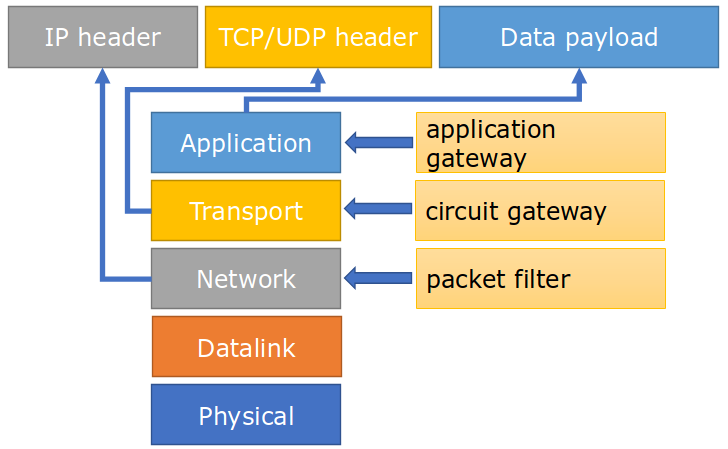
\includegraphics[width=0.8\linewidth]{chapters/11/images/controlli.png}
\end{figure}

\noindent Possiamo parlare di \textit{personal firewal} quando intendiamo una protezione 
orientata su un singolo host; è generalmente implementato come un filtro sw per 
proteggere il dispositivo da accessi indesiderati provenienti dall'esterno della rete.

\begin{figure}[H]
    \centering
    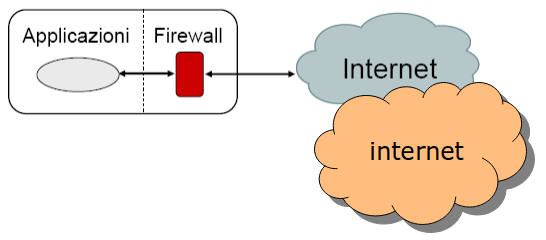
\includegraphics[width=0.6\linewidth]{chapters/11/images/personal-fw.png}
\end{figure}

\noindent Un \textit{firewall di rete} può anche essere una macchina dedicata che filtra tutto 
il traffico da e per una rete locale.

\begin{figure}[H]
    \centering
    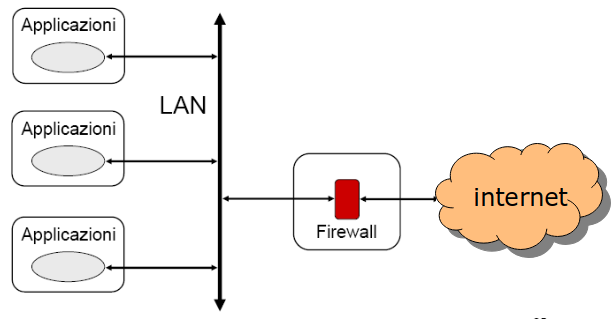
\includegraphics[width=0.6\linewidth]{chapters/11/images/fw.png}
\end{figure}


\subsection{Considerazioni architetturali}

Spesso i computer forniscono dei servizi che devono essere raggiungibili 
dall'esterno; allo stesso tempo, altri servizi devono essere protetti.
Per questa ragione la \textbf{rete protetta da un firewall viene divisa in due zone}:
\begin{itemize}
    \item \textbf{Rete pubblica:} è quel tratto di rete visibile da \textit{tutto il mondo}; ci possono essere situati
    un web server, mail server, \dots

    \noindent In gergo viene anche chiamata DMZ (\textit{de-militarized zone}), ovvero un tratto di rete in cui 
    il firewall permette l'accesso a tutti
    \item \textbf{Rete privata:} è la rete in cui i computer possono accedere ad internet ma non vengono
    visti dal \textit{mondo}
\end{itemize}

\begin{figure}[H]
    \centering
    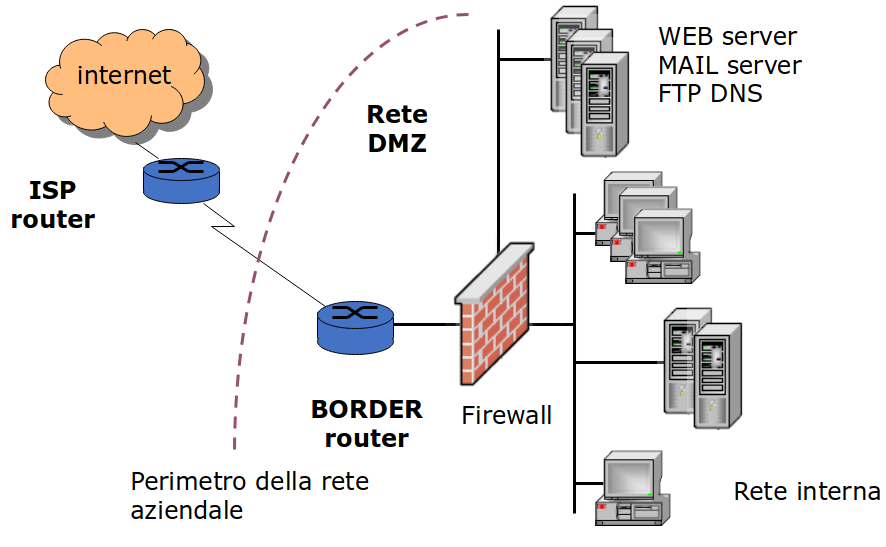
\includegraphics[width=1\linewidth]{chapters/11/images/zone.png}
\end{figure}

\noindent Sul firewall dovranno quindi essere installate tre \textit{interfacce di rete}:
\begin{itemize}
    \item una per il collegamento ad internet 
    \item una per la rete privata 
    \item una per la DMZ
\end{itemize}

\noindent Questa architettura prende il nome di \textbf{\textit{three-legged architecture}}.

\subsection{Protezione di rete}
\textbf{Tutto il traffico} tra la rete locale ed internet deve essere filtrato, mentre 
\textbf{solo il traffico autorizzato} può attraversare il firewall; i servizi 
necessari devono rimanere accessibili.

\noindent In fase di configurazione del firewall, si deve decidere la 
\textbf{politica di default} per i servizi di rete:
\begin{itemize}
    \item \textbf{\textit{Default deny:}} tutti i servizi non esplicitamente espressi sono negati 
    \item \textbf{\textit{Default allow:}} tutti i servizi non esplicitamente espressi sono permessi 
\end{itemize}

\noindent Il firewall permette di gestire una politica di accesso personalizzata per 
ogni sottorete ad esso collegata; solo i componenti esterni al firewall saranno 
senza protezione.

\noindent Si può inoltre gestire le connessioni tra le diverse interfacce del firewall 
(ad esempio, si può da internet alla DMZ ma non da internet alla rete privata).

$\rightarrow$ si può realizzare una separazione in zone aventi diverso grado di sicurezza 

\section{Packet Filtering}

\subsection{Static Stateless Packet Filtering (SPF)}
Il controllo del traffico è basato unicamente sulle informazioni contenute 
negli header dei singoli pacchetti.

\noindent I valori dei parametri degli header dei pacchetti vengono \textbf{confrontati 
con le regole definite in una ACL} (\textit{Access Control List}) e ammessi o scartati 
secondo il risultato del confronto.

$\rightarrow$ ogni pacchetto viene esaminato singolarmente, \textbf{indipendemente dagli altri pacchetti} precedenti 
o successivi

\noindent Il filtro scarta i datagrammi IP sulla base di:
\begin{itemize}
    \item tipo di servizio a cui il datagramma è destinato (porta TCP/UDP)
    \item indirizzo IP sorgente/destinazione 
    \item indirizzo MAC sorgente/destinazione 
    \item interfaccia di provenienza/destinazione 
\end{itemize}

\noindent Questa è la prima e più semplice tecnologia adottata per i sistemi di 
firewall. Nei sistemi odierni è stata superata dalla tecnologia di tipo \textit{stateful}, ma continua
ad essere usata nei sistemi di fascia bassa e nei router per la sua semplicità e per 
le ottime performance

\noindent Dato che \textit{Static} e \textit{Stateless} vanno di norma assieme, questo tipo di firewall
si può semplificare con \textbf{Static Packet Filter (SPF)}.

\subsection{Applicazioni di SPF}
Spesso, per alcuni servizi, si impone che le comunicazioni vengano regolate in 
modo tale che dalla rete interna si possa raggiungere l'esterno, ma non il contrario (ad esempio ping, SSH, \dots).

\subsubsection{Connessioni TCP}
Durante l'handshake, attraverso i FLAG dell'header TCP possiamo supportare la politica 
di sicurezza (ad esempio, solo da dentro a fuori).

\begin{figure}[H]
    \centering
    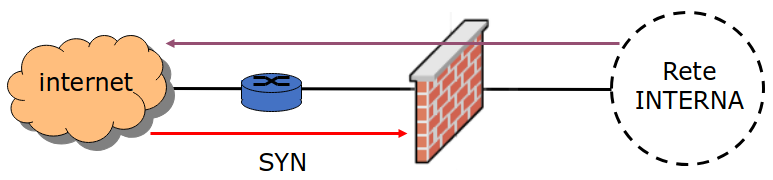
\includegraphics[width=0.8\linewidth]{chapters/11/images/spt-tcp.png}
\end{figure}

\subsection{Efficacia}
STP è capace di proteggere da:
\begin{itemize}
    \item attacchi elementari di \textbf{spoofing}
    \item \textbf{tentate connessioni}, tramite controllo degli IP, porte di destinazione e flag TCP 
    \item \textbf{traffico ICMP malevolo}
\end{itemize}

\noindent $\rightarrow$ è utile se configurato su un router come primo livello di protezione perimetrale; protegge solo da 
tecniche di attacco non sofisticate

\subsection{Stateful Filtering}
Un packet filter può essere \textit{stateless} o \textit{stateful}. Questa separazione 
ormai è più teorica che pratica, dato che tutte le implementazioni di SPF offrono anche qualche tipo 
di \textit{protocol inspection}, per cui sono \textbf{multilayer stateful firewall}.

\subsubsection{Protocol inspection}
La \textbf{stateful} inspection è quel processo per cui ogni singola connessione autorizzata 
viene registrata dal firewall in una apposita tabella, la cosidetta \textbf{connection} o \textbf{state table}:
\begin{itemize}
    \item oltre all'IP sorgente e di destinazione, vengono registrati tanti altri dati, come 
    il protocollo, le porte, i flag, sequence number \dots
\end{itemize}

$\rightarrow$ è difficile per un hacker inserirsi in una connessione stabilita (\textit{session hijacking})

\noindent Nella pratica, ogni volta che un pacchetto arriva al firewall, viene verificato 
se esso fa parte di una connessione precedentemente stabilita:
\begin{itemize}
    \item in caso affermativo, viene lasciato passare senza ulteriori controlli 
    \item altrimenti subisce i controlli di un normale pacchetto in ingresso
\end{itemize}

\subsection{Considerazioni sul packet filtering}
Anche con la migliore configurazione il packet filter \textbf{non verifica 
il contenuto dei pacchetti}, per cui non può bloccare virus; inoltre, ha problemi
con i protocolli che allocano le porte in maniera dinamica come FTP.

\section{Access Control List}
Le ACL definiscono regole per il filtraggio statico dei pacchetti in transito. La semantica 
è ACCEPT/DENY, ed utilizzano un criterio \textit{top-down} di filtraggio:
\begin{itemize}
    \item la prima regola che viene verificata produce la decisione sul pacchetto
    \item il test del pacchetto continua fino a che una regola corrisponde alle caratteristiche 
    del pacchetto oppure fino a che la lista di regole termina 
    \item di norma esiste una regola di default
    \begin{itemize}
        \item Default Permit 
        \item Default Deny 
    \end{itemize}
\end{itemize}

\noindent Le ACL lavorano al livello \textit{network} della pila ISO/OSI.

\subsection{Standard ACL}
Le \textit{standard ACL} sono numerate tra 0 e 99, filtrano \textbf{solo} gli 
indirizzi \textbf{IP sorgente}.

\begin{center}
    \texttt{Access-list numero azione sorgente [wild card] | any}
\end{center}

\begin{itemize}
    \item Numero: da 0 a 99 
    \item Azione: \textit{permit} o \textit{deny}
    \item Sorgente: indirizzo IP sorgente 
    \item Wild card: determina la parte dell'indirizzo IP da verificare e quella di ignorare;
    è simile alla netmask, ma ha una semantica dei valori invertita:
    \begin{itemize}
        \item valore binario 1: bit dell'indirizzo IP non deve essere verificato
        \item valore binario 0: bit dell'indirizzo IP deve essere verificato 
    \end{itemize}
    \item Any: qualunque valore
\end{itemize}

\subsubsection{Esempi}
\begin{itemize}
    \item \texttt{Access-list 17 permit host 192.168.1.100}
    \begin{itemize}
        \item la keyword \texttt{host} si usa quando si indica un indirizzo IP unico; analogo 
        ad usare wildcard 0.0.0.0
    \end{itemize}
    \item \texttt{Access-list 17 deny 192.168.1.0 0.0.0.255}
    \item \texttt{Access-list 17 permit any}
    \begin{itemize}
        \item la regola di default viene fatta usando \texttt{permit any} oppure \texttt{deny any}
    \end{itemize}
\end{itemize}

\noindent Le ACL possono essere categorizzate in due:
\begin{itemize}
    \item \textbf{Ingress firewall:} controllo sui collegamenti \textit{incoming}, tipicamente verso 
    servizi offerti all'esterno
    \item \textbf{Egress firewall:} controllo sui collegamenti \textit{outgoing}; controllo sull'attività del personale
\end{itemize}

\noindent Questa distinzione è facile per i servizi orientati al canale (TCP), più difficile 
per quelli basati su datagrammi (UDP, ICMP).

\noindent Secondo lo standard RFC 2827, ogni pacchetto che abbandona la rete dovrebbe avere come IP sorgente 
un indirizzo della rete locale, mentre ogni pacchetto in entrata non dovrebbe mai avere come sorgente 
un IP nella rete locale; un esempio di ACL egress può essere:

\begin{lstlisting}
    Access-list 14 permit <rete interna> <wiild card>
    Access-list 14 deny any
\end{lstlisting}

\subsection{Extended ACL}
\begin{center}
    \texttt{Access-list numero azione tipo sorgente [wild card] opzioni
    destinazione [wild card] [log]}
\end{center}

\begin{itemize}
    \item Numero: da 100 a 199 
    \item Azione: Permit/Deny
    \item Tipo: IP, UDP o TCP 
    \item Sorgente: indirizzo IP sorgente 
    \item Opzioni: porte TCP/UDP, Tipo/Codice ICMP, operatori speciali:
    \begin{itemize}
        \item eq: \textit{equal} 
        \item neq: \textit{not equal}
        \item gt: \textit{greater than} 
        \item lt: \textit{less than}
    \end{itemize}
    \item Log: scrive un messaggio in un log per ogni pacchetto verificato da una regola
\end{itemize}

\subsubsection{Esempi}
\begin{itemize}
    \item \texttt{Access-list 101 permit tcp 192.168.2.0 0.0.0.255 any eq 23}
    \item \texttt{Access-list 101 permit tcp 192.168.2.0 0.0.0.255 any eq ftp}
\end{itemize}

\noindent Come si può vedere, gli operatori logici possono essere usati sia con numeri di 
porta che con keyword. 

\noindent È possibile usare \texttt{eq established} per accettare unicamente delle 
connessioni TCP già stabilite.

\subsection{ACL e interfacce}
Una volta definita una ACL, è necessario \textbf{associarla ad un'interfaccia}
del dispositivo di rete:

\begin{center}
    \texttt{ip access-group accessListNumber \{in|out\}}
\end{center}

\begin{itemize}
    \item accessListNumber: indica il numero dell'ACL che deve essere legata all'interfaccia 
    \item in|out: specifica se l'ACL vada applicata al traffico in entrata o in uscita
\end{itemize}

\newpage
\section{ACL e protocolli applicativi}

\subsection{Esempio}
Si vuole negare all'host B l'accesso al Server FTP e allo stesso tempo negare all'host C 
qualsiasi accesso alla rete 172.16.3.0

\begin{figure}[H]
    \centering
    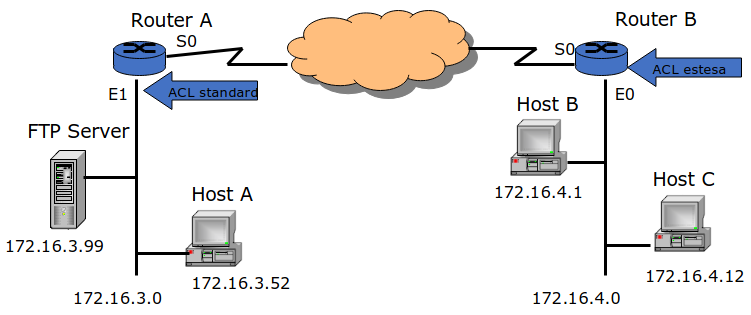
\includegraphics[width=1\linewidth]{chapters/11/images/esempio.png}
\end{figure}

\begin{lstlisting}
    access-list 1 deny host 172.16.4.12 
    access-list 1 permit any
    interface ethernet 1 (E1)
    ip access-group 1

    access-list 101 deny tcp host 172.16.4.1 172.16.3.0 0.0.0.255 eq ftp 
    access-list 101 permit ip 172.16.4.0 0.0.0.255 any 
    interface ethernet 0 (E0)
    ip access-group 101
\end{lstlisting}

\subsection{Formalismo}
Una ACL Static Packet Filter è definita da una tabella come la seguente:

\begin{figure}[H]
    \centering
    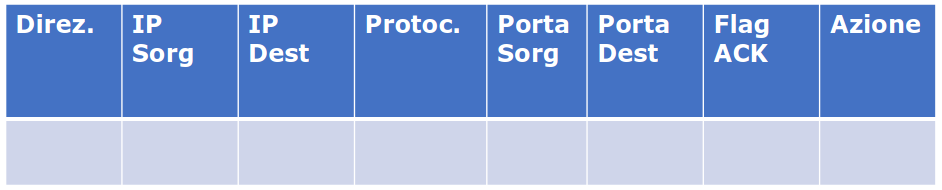
\includegraphics[width=1\linewidth]{chapters/11/images/tabella.png}
\end{figure}

\noindent È molto diffuso l'uso di variabili alle quali assegnare dei parametri, tipicamente indirizzi IP e sottoreti. L'utilizzo delle variabili 
al posto dei valori permette di:
\begin{itemize}
    \item separare la definizione dei valori dalle definizione della politica del firewall
    \item si possono modificare i valori senza modificare la politica stessa
\end{itemize}

\subsection{Esempio con Telnet}
Vogliamo autorizzare solo connessioni Telnet dall'interno della rete aziendale verso 
l'esterno (assegnato alla porta 23).

\begin{figure}[H]
    \centering
    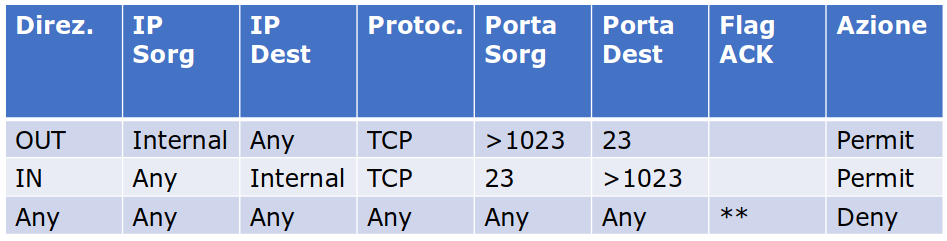
\includegraphics[width=1\linewidth]{chapters/11/images/telnet1.png}
\end{figure}

\noindent Filtrare il traffico solo sulle porte sorgente e destianzione può 
portare ad una politica troppo permissiva. Ad esempio, la regola 

\begin{center}
    \texttt{IN any Internal TCP 23 >1023 Permit} 
\end{center}

\noindent permette connessioni generate da qualunque host esterno e dirette a qualunque host interno 
aventi porta sorgente 23/TCP e porta destinataria >1023

\noindent Sappiamo che i pacchetti provenienti dall'esterno della rete sono solo
le risposte del server. Possiamo limitare la politica ai soli server utilizzati:

\begin{figure}[H]
    \centering
    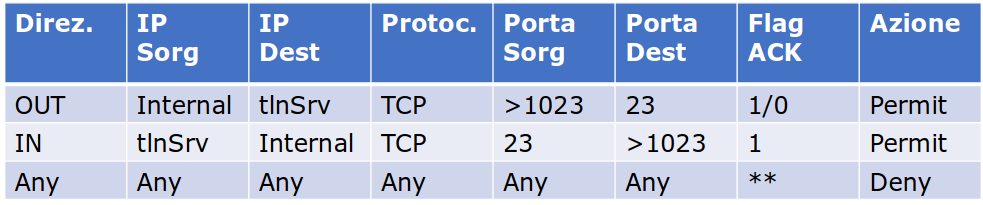
\includegraphics[width=1\linewidth]{chapters/11/images/telnet2.png}
\end{figure}

\noindent Usiamo ACK:
\begin{itemize}
    \item 1/0 quando IP sorgente stabilisce la connessione verso IP destinatario 
    \item 1 quanod IP sorgente risponde all'IP destinatario
\end{itemize}


\noindent In generale, \textbf{la politica di un firewall deve essere la più stringente 
possibile; è un errore definire una politica più \textit{lasca} dello stretto necessario}.


